\documentclass[10pt,a4paper]{article}

\usepackage[latin1]{inputenc}
\usepackage{amsmath}
\usepackage{amsfonts}
\usepackage{amssymb}
\usepackage{graphicx}
\usepackage{color, colortbl}
\usepackage{fancyhdr}

\pagestyle{fancy}
\fancyhf{}

\rhead{\leftmark}
\lhead{Using Infer}
\rfoot{Page \thepage}

%%%%% COMMANDS
\newcommand{\exercise}[1]{\vspace{1cm} \color{blue} \framebox[1.1\width]{\textbf{\textsc{Exercise:} #1}}\color{black}}

\newcommand{\todo}[1]{\color{red} \textbf{\textsc{TODO:} #1 }\color{black}}

\newcommand{\dothis}[1]{\vspace{1cm} \color{blue} \framebox[1.1\width]{\textbf{\textsc{Complete the Following:} #1}}\color{black}}

\newcommand{\note}[1]{\noindent\fbox{\parbox{\textwidth}{\textbf{NOTE:} #1} }}
%%%%%%%%%%%%%%%

\author{Shane Magrath}
\title{Using Infer to Find Bugs: \\Lab Directed Training}

\begin{document}

\maketitle
\section{Introduction}

\subsection{Overview}

\textit{Infer} is a static analysis tool whose purpose
is to find bugs in code that normal code compilation won't find.
Infer is owned by Facebook who open-sourced the tool in 2015.
Since then the tool has been used by quite a few Internet scale companies
such as Uber, Spotify, Mozilla as well as Facebook to find thousands of bugs 
a month in their code bases. It has a good reputation.

\textit{Infer} has a significant foundation in advanced program analysis techniques
developed by academia. This includes theories such as \textit{Abstract Interpretation} and 
\textit{Separation Logic}. You do not need to understand these theories to use the tool
but they are the reason why the tool is effective in finding non-trivial bugs 
that the compiler doesn't catch. The cost however for this ability is that the
tool can take considerable resources to run in terms of memory and compute power.

\textit{Infer} can analyse C, C++, Objective-C and Java code. Not surprisingly
these are languages that matter a lot to Facebook: mobile applications and backend
server systems. In this training we focus on C and C++ code-bases. To be able to analyse
code with Infer you must be able to compile and build it. The reason for this is
that Infer captures many of the front-end compilation data-structures in order
for it to perform the advanced analyses it applies.

The bug reports generated by a static analysis tool such as Infer differ from 
the bugs found by other techniques from dynamic analysis. With dynamic analysis
techniques such as fuzzing, the bugs mostly are true positives. 
The reason is simple: an actual execution that results in a failure reveals
that the bug is not just theoretically possible but actually exists.

In contrast static analysis attempts to consider not just the space of \textit{actual} executions
but the much larger space of \textit{all possible} executions.
However to make this computation feasible static analysis techniques use
\textbf{over-approximation strategies} to reduce the size of the analysis space. 
The price you pay for computability is a reduction in the precision of the
analysis. It is important to understand this when inspecting Infer's bug reports.

\subsection{Learning Outcomes}

Upon completion of this course, the student will be able to:
\begin{itemize}
	\itemsep0em
\item Understand static analysis and its applications and limitations to bug finding
\item Install Infer on a Linux machine
\item Run Infer against a C/C++ source code targets
\item Enable different Infer checkers, including \textit{Inferbo} and \textit{Quandary}
\item Generate Infer HTML and JSON bug reports
\item Read and understand Infer bug reports for code audit purposes
\item Understand and develop Infer linters for syntactic bug finding using Infer's AL language 
\item How to generate Call Flow Graphs (CFGs) and other front end compilation data for target code understanding and debugging
\item How to use Infer with CMake using a \textit{compilation database}
\end{itemize}

\subsection{Pre-requisites}
\begin{itemize}
\item Knowledge and some proficiency in C and C++ coding, compilation and debugging
\item Knowledge of C/C++ bug classes and Code Review principles and practice (\todo{list some})
\item Knowledge of Linux Shell commands and operating system operation
\end{itemize}

\subsection{Lab Exercises}

\begin{itemize}
\item \textbf{Lab ONE}: Basic analysis of a target
\item \textbf{Lab TWO}: \textit{Inferbo}: Buffer Overflow and Integer Bugs
\item \textbf{Lab THREE}: \textit{Quandary}: \\Static Taint Analysis and Command Injection Bugs
\item \textbf{Lab FOUR}: \textit{Linters}: How to write a linter in AL
\end{itemize}
\section{Getting Started}

\subsection{Infer Installation Using Docker}

This section we are going to install Infer and the three audit targets
using Docker.
The purpose of using Docker is to avoid spending unnecessary time 
on resolving configuration and dependency issues with the tool and 
the various targets.
However in the appendix we show how to install and configure Infer 
natively for a Linux system.

These notes are on how to use Docker to do this lab. 

\dothis{Install and Run the Infer Docker}


\noindent From the root of the lab repo: 

\begin{verbatim}
# Create our lab directory to share files with host
mkdir ./lab

# Install and configure Docker on Ubuntu
sudo apt install docker.io
sudo usermod -aG docker ${USER}
su - ${USER}
git clone https://github.com/smagrath/infer-training
cd infer-training

# Build a docker image from the Dockerfile in sub-dir ```lab```
# Tag it infer-training 
docker build -t infer-training .

# Create a new container based on the image above 
# mount the host sub-dir ```content``` into the container 
docker create -it -v `pwd`/lab:/root/lab --name infer infer-training

# Boot the container
docker start infer

# Run a terminal in the container
docker exec -it infer /bin/bash

# In the Docker terminal run the configure script.
# This script pulls down and "patches" the audit targets.
cd lab
./configure.sh
\end{verbatim}

You now have a running Docker container with Infer and the three audit targets
installed and configured along with their dependencies. 
Also, the host and the Docker container share a common sub-directory on
which allows files to be transferred to the host machine.
This shared directory is the \verb|./lab| directory of this training repo. 
The main reason for doing this is so we can use the host OS's web browser
to view the Infer reports and other data files.
The Docker image has no GUI support.

When you're finished with your Docker image complete the following:

\begin{verbatim}
# docker stop infer
# docker rm infer
# docker rmi infer-training
\end{verbatim}

This will stop the Docker container and delete the Infer image from the host machine.

\section{Audit Targets}

We will use the following three Linux games to explore Infer.

\begin{itemize}
	\itemsep0em 
	\item \textbf{Angband} - \verb|https://rephial.org/|
	\item \textbf{Skynet} - \verb|https://github.com/cloudwu/skynet|
	\item \textbf{BSDGames} - \verb|https://github.com/vattam/BSDGames|
\end{itemize}

The targets were chosen because together they exhibit a good diversity of bugs
and have modest build and analysis requirements. 
Some targets because of size and complexity issues require large amounts of 
memory (i.e. more than 16 GB) and compute time (i.e. more than 10 minutes) which is not appropriate
for the typical resources available for this lab.

The Docker container has the build systems, source code and library dependencies
already installed. 
However we have included in the Appendix the process to build the targets 
from scratch for the purpose of being analysed by Infer.

Infer uses Clang and therefore the targets must be buildable with Clang.
Moreover Infer hooks several build tools such as \verb|make|, however
it can take a bit of effort to get Infer to work with tools like \verb|CMake|.
We look at how this down in TODO.

In practice you should not under-estimate how much effort is required to 
properly prepare a target for Infer. Your goal is to maximise analysis
coverage which means that you need to configure the target build system 
to use as many features and libraries as possible. 
Recursively, you should consider analysing the source code of the library dependencies
as well.

In the following subsections we will complete the build configuration for the
targets.
We could have scripted this work however this is not helpful to you.
Part of using Infer effectively is understanding and controlling the build
process of the audit targets intimately.

\subsection{Angband}

In the Docker terminal:

\dothis{Verify you can build Angband}


\begin{verbatim}
$ cd angband-4.2.0
$ CC=clang CXX=clang++ ./configure --enable-sdl2
$ make
\end{verbatim}

The build should complete successfully with no errors.

\subsection{Skynet}

We are going to build \verb|Skynet|. 
I've always wanted to build Skynet.
I've always wanted to ride a Harley-Davidson, wear a leather jacket and 
wield a sawn-off shotgun. I look cool in sun-glasses too.

To build Skynet we need to explicitly identify that it is a \verb|linux| 
build configuration. You will need to remember this throughout the course.

In the Docker terminal:

\dothis{Verify you can build Skynet}

\begin{verbatim}
$ cd skynet
$ CC=clang CXX=clang++ make linux
\end{verbatim}

The build should complete successfully with no errors.

\subsection{BSDGames}

We will need to manually edit (using Vim) the \verb|Makeconfig| file to use Clang instead of GCC.
The usual method of setting environment variables is ineffective.

In the Docker terminal:

\dothis{Verify you can build BSDGames}

\begin{verbatim}
$ cd bsdgames
$ ./configure
$ vim ./Makeconfig
# --> change the compilers from GCC/G++ to Clang/Clang++
$ make
\end{verbatim}

The build should complete successfully with no errors however you will 
see plenty of warnings. It's old code.
\section{Lab One: Basic Usage of Infer}

The purpose of this lab is to:
\begin{itemize}
	\itemsep0em
	\item Verify that your Infer installation is working properly by producing \textit{basic reports}.
	\item Generate both HTML and JSON bug reports.
	\item Examine the basic report in a browser and gain familiarity with what basic bug classes 
	Infer finds and how they are reported.
	\item Gain proficiency understanding Infer's reported bugs.
\end{itemize} 

\dothis{Basic Infer Usage}

\vspace{0.5cm}

\textbf{For each of the three targets perform the following operations:}

\begin{enumerate}
	\itemsep0em
	\item In the repo root directory, type:\\
	\verb|make clean|, and then \\
	\verb|infer run --keep-going -- make -j6|\\
    The option \verb|--keep-going| forces the process to keep going when Infer encounters errors. Always recommended. Also, always make sure you have a \verb|make clean| state before analysis.    
    Infer analysis can take some time to complete. Typically:
    \begin{itemize}
    	\item \textbf{Angband}: about 7 minutes
    	\item \textbf{SkyNet}: about 1 minute
    	\item \textbf{BSDGames}: about 3 minutes
    \end{itemize}
	\item When the Infer analysis is complete you will see on screen a summary. 
	Verify that it looks something like the following:\\
	\begin{verbatim}		
		...too many issues to display (limit=10 exceeded), please see
/home/dstcyber/workspace/audit/BSDGames/infer-out/bugs.txt 
or run `infer-explore` for the remaining issues.
		
		Summary of the reports
		
		UNINITIALIZED_VALUE: 100
		DEAD_STORE: 37
		NULL_DEREFERENCE: 34
		RESOURCE_LEAK: 10
		MEMORY_LEAK: 5
		USE_AFTER_FREE: 1		
	\end{verbatim}
	\item Verify that Infer has created a sub-directory containing all its analysis:\\
	\verb|# cd ./infer-out|\\
	Have a look in this directory. If you want to re-run the analysis I tend to just 
	delete the \verb|./infer-out| directory tree and start again. This is not always necessary
	and in fact it can save considerable time if you don't but don't be afraid to delete it if you want 
	to start again.
	\item Inspect the JSON report file:\\
	\verb|# vim ./infer-out/report.json|\\
    You may want to examine this in VSCode which can pretty print format the JSON data. 
	\item Generate a HTML report file:\\
	\verb|# infer explore --html| \\
	You should see something like the following:
	\begin{verbatim}
		Detected GitHub project vattam/BSDGames
		Saved html report in:
		./infer-out/report.html/index.html
	\end{verbatim}
	\item Open the HTML report in a browser \textbf{from your host}:\\
	\verb|# xdg-open ./infer-out/report.html/index.html|
\end{enumerate}

When you open the report in a browser you should see something similar to Figure \ref{fig:screen-one}.
It's not a very attractive looking report  :-)

\begin{figure}
	\centering
	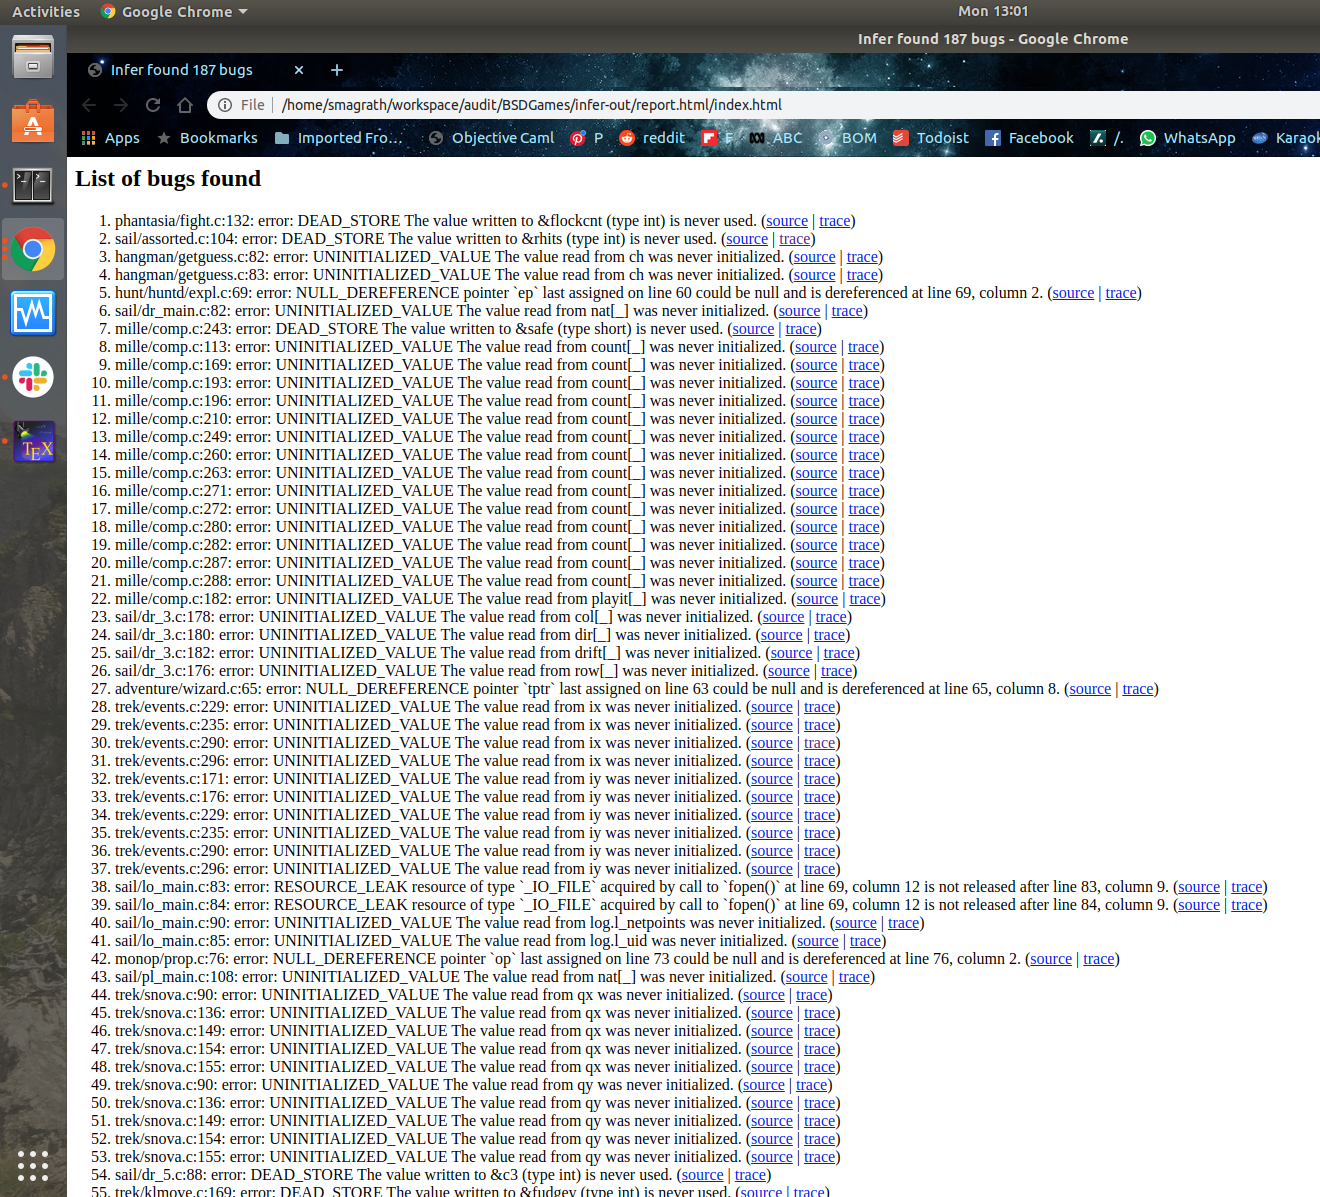
\includegraphics[width=\linewidth]{./img/screen-one}
	\caption[Basic Report]{Basic Infer Report for BSDGames}
	\label{fig:screen-one}
\end{figure}

\vspace{1cm}

\subsection{Examining Bug Reports}

It is very common to get a large number of bug reports when using Infer. 
It is important to have a strategy when deciding which reports to look at.
Your strategy will depend on what your goals are and will improve with experience
in using the tool. Not all bug reports are of equal value.

Your strategy may include factors such as:
\begin{itemize}
	\item Which bug classes are of the most interest to you;
	\item Which functions and translation units (files) are most important;
	\item How much time you have :-)
\end{itemize}

In general, your analysis process will need to examine the \textit{trace} of a bug report.
The trace is a \textit{almost} human readable description of why Infer thinks it has found a bug.
When looking at the trace the most important parts are the \textit{first few lines and the last few lines}. The first line declares what the bug is and where it is. 
The last few lines point to the specific problem point. 
If the trace has reasonable length then the intermediate parts of the trace 
are the execution path which causes the problem. 

\exercise{Click on a sample of the following bug classes:}

\begin{itemize}
	\itemsep0em
	\item \verb|DEAD_STORE|
	\item \verb|NULL_DEREFERENCE|
	\item \verb|UNINITIALIZED_VALUE|
	\item \verb|RESOURCE_LEAK|
	\item \verb|NULL_DEREFERENCE|
	\item \verb|MEMORY_LEAK|
	\item \verb|USE_AFTER_FREE|
\end{itemize}

\textbf{For each of the bug classes consider the following:}
\begin{enumerate}
	\item Is the bug report correct?
	\item If not, can you think of a reason why it failed? \\
	This is an important skill for learning how to quickly dismiss bug reports.
\end{enumerate}


In particular examine the following interesting \textit{specific} bugs:
\begin{itemize}
    \item See the whiteboard :-)
\end{itemize}


However it is important that you learn how to:
\begin{enumerate}
	\item efficiently triage the report when you have a lot of records;
	\item efficiently follow the reasoning of an Infer report trace. 
\end{enumerate}

\subsection{What Have We Learnt So Far?}

\begin{enumerate}
	\itemsep0em
	\item How to install and run Infer using the default checkers;
	\item How to check the Infer man page and online documentation;
	\item The location and contents of the Infer analysis in \verb|./infer-out|
	\item How to find the JSON bug report;
	\item How to generate a HTML report of the bugs found;
	\item How to read the bug traces for a variety of bug classes;
\end{enumerate}

\subsection{What Next?}

In the next lab we will be looking at Integer bugs and Buffer-overflows.



\section{Lab Two: Inferbo}

The purpose of this lab is to use Infer to find:
\begin{itemize}
	\itemsep0em
	\item \textbf{Integer Bugs} - overflows, sign vs unsigned bugs, sign extension bugs etc;
	\item \textbf{Buffer Overflows}: memory corruption bugs	
\end{itemize}

Infer uses an experimental checker called ``Inferbo'' to do this analysis. 
This checker uses Abstract Interpretation Theory to analyse the effects of integer expressions
and their application to memory structures such as arrays.

\subsection{Running Inferbo}

Like all checkers , we can run \textit{Inferbo} as an additional analysis \textit{or} on its own.

\begin{itemize}
	\item As an \textbf{additional} checker: \\
	\verb|# infer run --bufferoverun -- make |
	\item \textbf{Inferbo only}:\\
	\verb|# infer run --bufferoverrun-only -- make |	
\end{itemize}

\exercise{Working with Inferbo}

\vspace{0.5cm}
For each of the targets run Inferbo on its own and generate HTML bug reports.
Open each of the bug reports and examine the various bug \textit{classes}.

\textbf{Remember: }
\begin{itemize}
	\item Delete any previous Infer data:\\
	\verb|# rm -rf ./infer-out| \\
	Otherwise the results of previous analysis may leak into the reports.
	\item Clean the build:\\
	\verb|# make clean|\\
    Otherwise Infer won't analyze anything.
\end{itemize}

You should see a summary like:
\begin{verbatim}
	...	
	
	Summary of the reports
	
	BUFFER_OVERRUN_L3: 14
	BUFFER_OVERRUN_L2: 9
	INFERBO_ALLOC_MAY_BE_BIG: 9
	INTEGER_OVERFLOW_L2: 8
	INFERBO_ALLOC_IS_ZERO: 4
	INFERBO_ALLOC_MAY_BE_NEGATIVE: 1
	INTEGER_OVERFLOW_R2: 1
	BUFFER_OVERRUN_L1: 1	
\end{verbatim}

Notice that the various bug classes have suffixes like ``L1'' and ``L3''. 
I'm not exactly sure what they mean but I strongly suspect that they relate 
to specific class variations of a bug that is being reported.

A few specific things to know:
\begin{itemize}
	\itemsep0em
	\item \textbf{Understanding Traces}: The first few lines of a \verb|BUFFER_OVERRUN| trace are very important. It tells you why it thinks there is a memory error. For example:\\
	\verb|Offset: [3, 18] Size: 16| is interpreted as the buffer is sized 16 but the index range is predicted by analysis to vary between 3 and 18. 
	\item \textbf{Confusing arithmetic}: Some maths expressions seem to confuse Infer and therefore
	the range calculations seem to be in error. In particular bit operations and union structures seem a problem.
	\item \textbf{Precision}: Remember this is \textit{static} analysis. Runtime execution may
	be protective of the problem identified. However, a lot of bug reports would be eliminated if
	the source code had proper bounds checking in place.
\end{itemize}

In particular examine the following interesting \textit{specific} bugs:
\begin{itemize}
	\item See whiteboard :-)
\end{itemize}

\subsection{What have we learnt so far?}

In my experience the Inferbo reports are always worth thinking through. 
They often can be eliminated with simple bounds checking at the identified problem site.

\subsection{What Next?}

The next section we will look at \textit{Quandary} - a static source-sink or taint checker.


\section{Lab Three: Quandary}

Quandary is an experimental checker in Infer. 
It performs \textit{static taint analysis}, also called \textit{source-sink} analysis.
The essential idea is that you can specify a \textit{data-flow} between a
\begin{itemize}
	\item \textbf{source} function - that is the return value of the function;
	\item \textbf{sink} function: to a specific argument or any argument of that function.
\end{itemize} 

This is a really interesting checker from a security auditing perspective. 
For example, it allows you to specify a test from attacker-controlled data 
(for example, environment variables) to security sensitive functions (for example, \texttt{execve} functions).

For technical reasons this is also an impressive checker because it does this 
analysis \textit{statically} and efficiently.

\subsection{Running Quandary}

Like all checkers , we can run \textit{Quandary} as an additional analysis \textit{or} on its own.

\begin{itemize}
	\item As an \textbf{additional} checker: \\
	\verb|# infer run --quandary --keep-going -- make |
	\item \textbf{Inferbo only}:\\
	\verb|# infer run --quandary-only --keep-going -- make |	
\end{itemize}

\exercise{Working with Quandary - Part One}

\vspace{0.5cm}
For each of the targets run Quandary on its own and generate HTML bug reports.
Open each of the bug reports and examine the various bug \textit{classes}.
Start with \texttt{BSDGames} in this example.

\textbf{Remember: }
\begin{itemize}
	\item Delete any previous Infer data:\\
	\verb|# rm -rf ./infer-out| \\
	Otherwise the results of previous analysis may leak into the reports.
	\item Clean the build:\\
	\verb|# make clean|\\
	Otherwise Infer won't analyze anything.
\end{itemize}

You should see a summary like:

\begin{verbatim}
...
Summary of the reports

SHELL_INJECTION: 4
\end{verbatim}

By default, Quandary looks for data-flows between environment variables (as returned by \texttt{gentenv()})
and the \texttt{execve()} functions. These data-flows represent command injection vulnerabilities if there
is no sanitisation of the environment variable.

\exercise{Working with Quandary - Part Two}

\vspace{0.5cm}
In this example we are going to define our own source-sink data-flow we are interested in.

\begin{itemize}
	\item Create the following JSON file: \texttt{.inferconfig} in the root of the target 
	repo.
	\item Insert the following contents:\\
	\noindent\begin{verbatim}
    {
        "quandary-sources": [
        {
            "procedure": "getenv",
            "kind": "Logging"
        }
        ],
        "quandary-sinks": [
        {
            "procedure": "atoi",
            "kind": "Logging"
         }
         ]
    }	
	\end{verbatim}
	\item Re-run the Quandary analysis:\\
	\verb|# infer run --keep-going --quandary-only -- make |
\end{itemize}

\textbf{Remember: }
\begin{itemize}
	\item Delete any previous Infer data:\\
	\verb|# rm -rf ./infer-out| \\
	Otherwise the results of previous analysis may leak into the reports.
	\item Clean the build:\\
	\verb|# make clean|\\
	Otherwise Infer won't analyze anything.
\end{itemize}

You should see a summary like:

\begin{verbatim}
...
Summary of the reports

SHELL_INJECTION: 4
QUANDARY_TAINT_ERROR: 3
\end{verbatim}

In this example we have picked three examples of a data-flow between an environment variable
and a function we defined as interesting: \verb|atoi()|. This is an interesting flow because
the function \verb|atoi()| has no error handling and fails silently. 
If you click on the trace for these reports you should indeed see an actual data-flow analysis
that reveals a bug. In fact any use of the function \verb|atoi()| should be considered a bug
however when confronted with lots of bugs these ones found by Quandary should be prioritised.

It is also possible to be specific about \textit{which argument} of the sink function you want 
to trace. By default, a data-flow to \textit{any argument} of the sink function triggers a report.

\todo{show how to specify this flow}

\subsection{Review}

What have we learnt so far?

\begin{itemize}
	\item Quandary is a static taint tracing checker;
	\item Quandary finds by default potential \textit{command injection} vulnerabilities;
	\item How to create our own source-sink analyses using the JSON file \verb|.inferconfig|
\end{itemize}


\subsection{What Next?}

In the next section we are going to learn how to use Infer's \textit{linting} capabilities.
\section{Lab Four: Finding Syntactic Bugs}

\texttt{Linting} is the process of finding \textit{syntactic} problems in code.
For example, any use of the function \verb|strcpy()| is now considered unsafe
and should be replaced with a more robust string copy method. 
Searching for uses of this function is linting.

Infer has a robust linting capability. It uses a domain specific language
called "AL" which is very advanced. We are only going to cover the surface 
of what you can do with AL. In particular, you should look at the fairly
extensive documentation on AL here: \verb|https://fbinfer.com/docs/linters.html|
and at the linters that come with Infer by default - from the root of the Infer installation  
find them as follows:  \verb|find . -name "*.al"|.

\subsection{Creating a linter: Part One}

In this section we are going to create a very simple linter using AL 
to find the unsafe functions \verb|atoi()| and \verb|strcpy()|. 
These are just to obvious choices of potentially many functions you would want to audit.

\begin{itemize}
	\item Create the following file: \verb|mylinter.al|
	\item Add the following content: we will go through what this means presently.
	\begin{verbatim}
DEFINE-CHECKER UNSAFE_FUNCTION_USAGE = {
	LET isatoi = call_function(REGEXP("\\batoi"));
	SET report_when =
		isatoi;
	SET message = "Unsafe function usage - atoi()";
	SET suggestion = "See Reference - TODO";
	SET severity = "ERROR";
};

DEFINE-CHECKER UNSAFE_FUNCTION_USAGE = {
	LET isstrcpy = call_function(REGEXP("\\bstrcpy"));
	SET report_when =
		isstrcpy;
	SET message = "Unsafe function usage - strcpy()";
	SET suggestion = "See Reference - TODO";
	SET severity = "ERROR";
};
	\end{verbatim}
	\item For each of the targets, run Infer as follows using the command below.\\
	Remember to \verb|make clean| and remove any prior \verb|infer-out| directory.\\
	\verb|# infer run --keep-going --linters-only --linters-def-file mylinter.al -- make|
\end{itemize}

You should see something like the following:

\begin{verbatim}
...
Summary of the reports

UNSAFE_FUNCTION_USAGE: 21
\end{verbatim}

Create a HTML report and have look at some of the traces.

\subsection{Understanding AL}

AL is a pattern matching language that operates on Clang's \textit{Abstract Syntax Tree} (AST).
The type of pattern matching is called \textit{Computational Tree Logic} (CTL).
CTL is a way of specifying pattern matching on tree structures. 
See "AL Formulas" at \verb|https://fbinfer.com/docs/linters.html| for a detailed 
description of how to do this.

The AST is a tree of the syntactic structure of the compiled source code produced by Clang.
Therefore we need to specify the syntactic pattern we are interested in finding in the AST
in terms of AL formulas. We will look at this in a moment.

Linting in AL consists of specifying one or more checkers. 
A checker consists of
\begin{itemize}
	\item One or more \textbf{formulas} that are triggered by a syntactic pattern in the AST;
	\item A \textbf{report rule} which causes a bug report to be raised. 
	The report rule consists of a combination of formulas that when true trigger the report;
	\item A \textbf{message} which summarises the issue;
	\item A \textbf{suggestion} of what to do about the issue;
	\item A \textbf{severity} to indicate how serious the issue is.
\end{itemize}

Lets analyse the following:

\begin{verbatim}
DEFINE-CHECKER UNSAFE_FUNCTION_USAGE = {
	LET isstrcpy = call_function(REGEXP("\\bstrcpy"));
	SET report_when =
		isstrcpy;
	SET message = "Unsafe function usage - strcpy()";
	SET suggestion = "See Reference - TODO";
	SET severity = "ERROR";
};
\end{verbatim}

Observe the following:
\begin{itemize}
	\itemsep0em
	\item We create the checker \verb|UNSAFE_FUNCTION_USAGE|
	\item We create a simple formula \verb|isstrcpy|
	\item We specify an AST pattern using \verb|call_function| which matches Clang's AST node for function call sites;
	\item We further specify a regex for function names which in our case matches \verb|strcpy|
	\item We specify a report to be raised when the \verb|isstrcpy| formulae is satisfied;
	\item The remaining lines are straight forward
\end{itemize}

This example demonstrates the basic structure of a linting checker. 
We will now look at a more involved example.

\subsection{Creating a Linter: Part Two}

In this section you will create a linter for the ``unsafe pointer accumulation 
using \verb|snprintf()|'' bug. Consider the following code:

\begin{verbatim}
#include <stdio.h>
#include <string.h>
#include <stdlib.h>
#include <stdbool.h>
    
#define SIZE 1024
    
/* Snippet to demonstrate the snprintf() pointer accumulation bug */
int main(int argc, char** argv) {
    char* buf = malloc(SIZE);
    char* text = NULL;
    char* q = text; //indexing ptr into text
    size_t len = 0; //of bytes written to buf 
    size_t tlen = 0; //length on source text
    
    text = malloc(SIZE);
    strcpy(text, "the quick brown fox jumped over the lazy dog");
    q = text;
    tlen = strlen(text);
    bool islast = false;
    printf("Input String = \"%s\"", text);

    while (!islast && ((q-text) < tlen) && (len < SIZE)) {
        char* t = index(q, ' '); //find the space
        if (t == NULL) {
            islast = true; //means we are at the last word
            t = text + tlen; //point at the end of the string 
        }
        size_t bytes = (t-q); //bytes to write
        *t = '\0'; //re-write the space so we can use the word
        //BUG: Unsafe pointer accummulation using snprintf()
        len += snprintf(buf+len, 100, "%7s: %3zu\n", q, bytes);
        q = t + 1; //next word
    }
    printf("Output: \n");
    printf("%s\n", buf);
    return 0;
}
    
\end{verbatim}

\noindent The bug we are interesting in finding involves this line:\\
\verb|len += snprintf(buf+len, 100, "%7s: %3zu\n", q, bytes);|

\noindent The source of the bug is assuming that the \verb|snprintf()| function 
returns the number of bytes written to the buffer. This function
does not make that guarantee - if the size of the string exceeds 100 bytes
in this example then the return value is the number of bytes that \textit{would} 
have been written - a larger number. Because we are in a loop the pointer value
into \verb|buf| is now wrong and we potentially could be writing into memory outside of 
\verb|buf|.

We could just grep for \verb|+= snprintf(| but this is not as robust nor integrated 
with Infer's bug reports. Therefore, we will make a linter to search for this bug pattern.

\subsubsection{Step One: Understanding the AST}

The first thing we need to do is understand the specific AST for this bug pattern.
We can get Clang to print the AST when it compiles the snippet above:

\verb|# clang -c -Xclang -ast-dump -fsyntax-only test_2.c|

You should see something similar to Figure \ref{fig:clang-ast}. The part of the AST
we are interested is highlighted. Study this closely and note the following:

\begin{itemize}
	\item The \verb|+=| accumulation operation is a \verb|CompoundAssignOperator| node in the AST.
	\item The function call involves \verb|CallExpr| node with a child node \verb|DeclRefExpr|
	whose value is \verb|snprintf|.
	\item Understand the parent-child relationships here in the AST.
\end{itemize}

\begin{figure}[t]
	\centering
	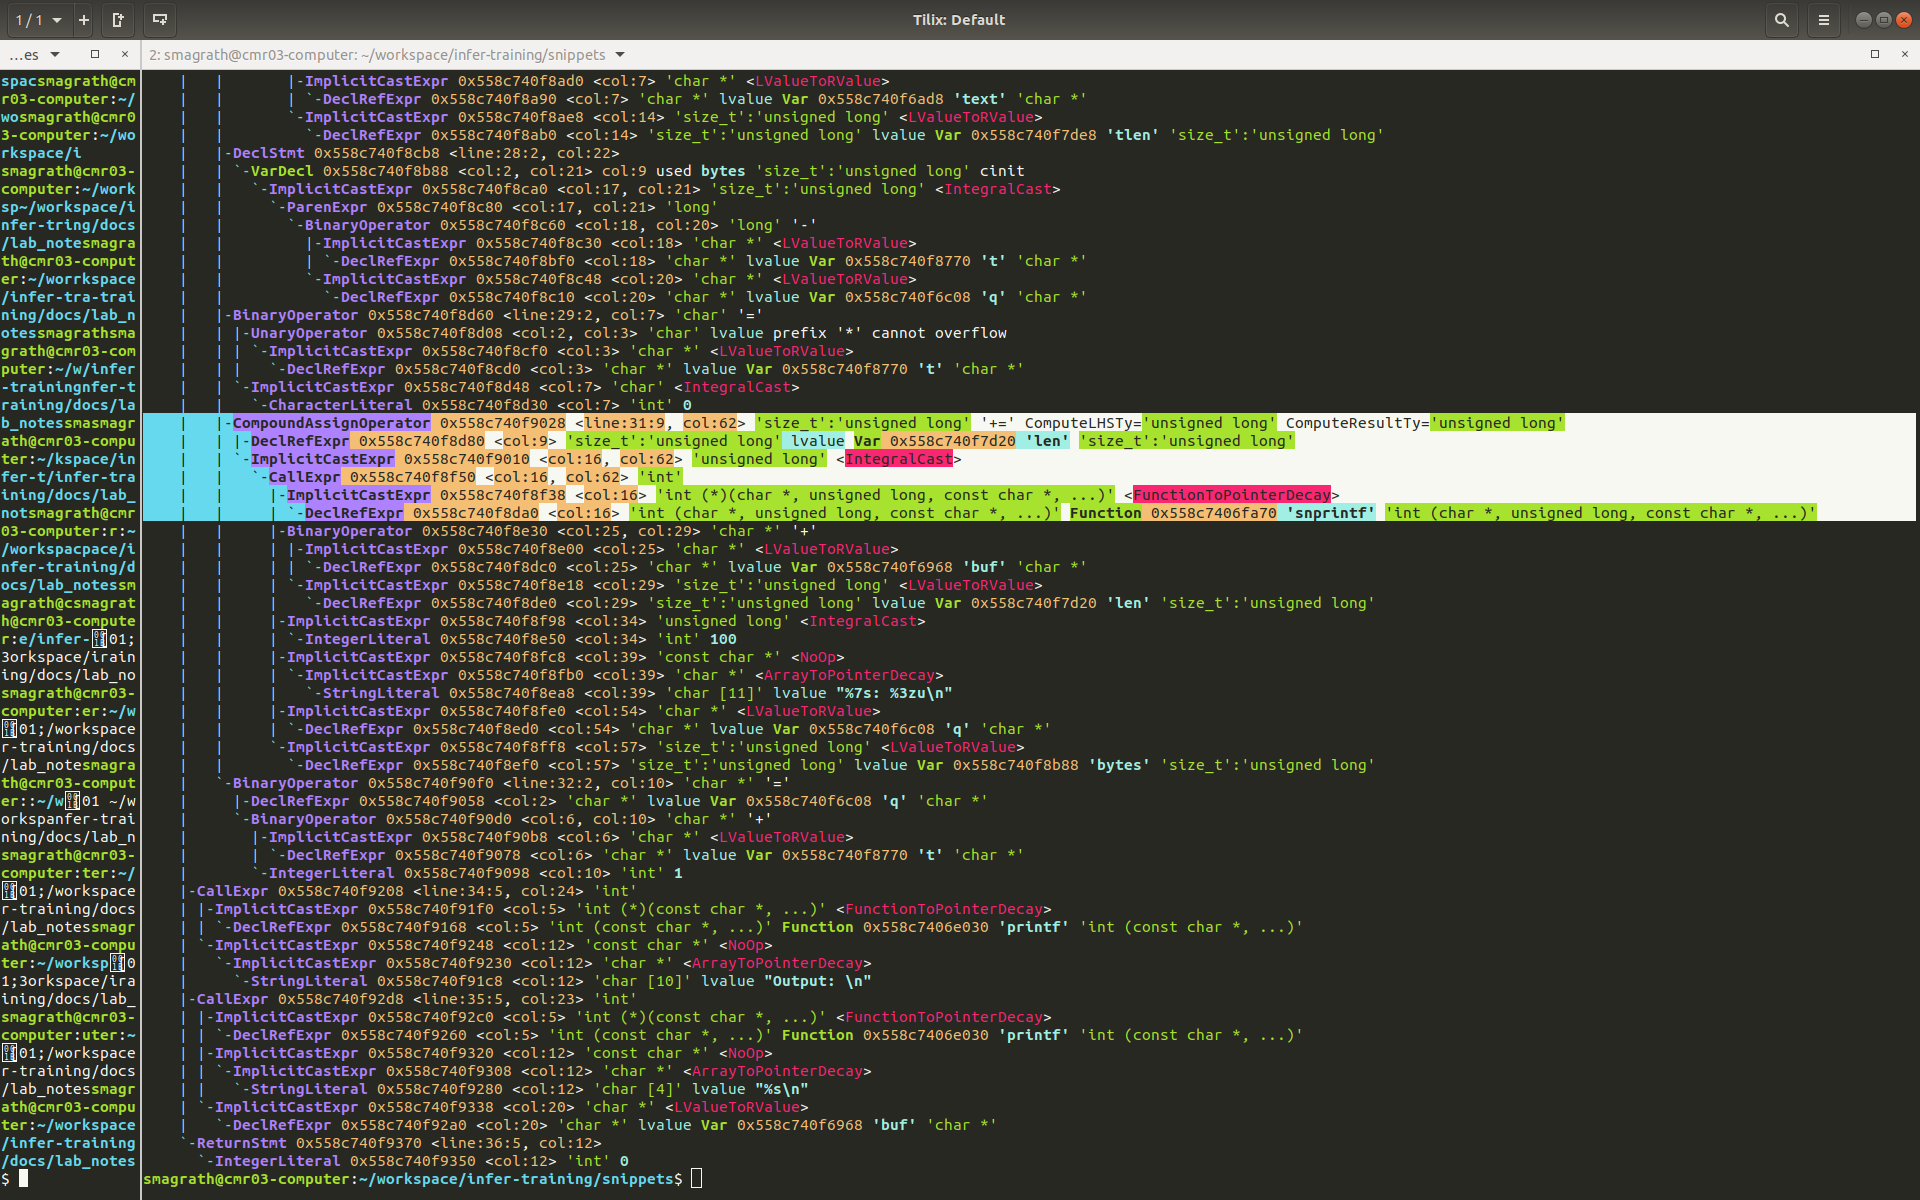
\includegraphics[width=\linewidth]{img/clang-ast}
	\caption[AST]{AST Screen shot}
	\label{fig:clang-ast}
\end{figure}

The next step is to specify a matching pattern that captures this syntactic structure.

\subsubsection{Step Two: Writing the Linter in AL}

There are various ways of writing this linter. 
We are going to write a simple version that over-approximates. That is, it can (and does) raise 
false positives. A more precise linter could be written but as we will see this has 
its own problems.

Add the following code to your \verb|mylinter.al| file.

\begin{verbatim}

DEFINE-CHECKER UNSAFE_SNPRINTF_ACCUMMULATION = {
    LET issnprintf = call_function(REGEXP("\\bsnprintf"));
    LET isaccum = is_node("CompoundAssignOperator");
    SET report_when = 
        issnprintf AND isaccum
    HOLDS-EVENTUALLY;
    SET message = "Possible Unsafe pointer accummulation using snprintf()";
    SET suggestion = "See Reference - TODO";
    SET severity = "ERROR";
};
\end{verbatim}

Note the following:
\begin{enumerate}
	\item We identify the \verb|snprintf| function using an AL \textit{predicate} called
	\verb|call_function|. This selects function call nodes in the AST. We further filter
	using a regular expression.
	\item We specifically select for \verb|CompoundAssignOperator| nodes in the AST.
	\item The particular tree pattern we want is where the call function is a child 
	of the \verb|CompoundAssignOperator| node. We can do this with the \verb|HOLDS-EVENTUALLY|
	CTL operator. Refer to the "AL Formulas" section of\\
	 \verb|https://fbinfer.com/docs/linters.html|. 
	In practice when developing linters you will need to become proficient with these formulas
	and linter debugging.
	\item Is this pattern completely correct to catch the bug we are after?	
\end{enumerate}

\exercise{Part Two: Linting for Unsafe Pointer Accumulation}

\begin{enumerate}
	\item Use Infer with the updated linter file for the code snippet.\\
	Verify that it identifies the problem line in the bug snippet.\\
	\verb|# infer run --linters-def-file ../mylinter.al -- clang -Wall -o test_2 test_2.c|
	\item For each of the targets run the linter and examine the bug reports:\\
	\verb|# infer run --keep-going --linters-only --linters-def-file ../mylinter.al -- make|
	\item You should find instances of false and true positives.\\ 
	Can you explain why the false positive occurred? 
	\item What are the limits of linting? Could you write a version of the \verb|snprintf()| bug 
	program that would not be caught by the linter?
\end{enumerate}

We are really only providing an introduction to Infer's linting capabilities here. 
You should examine the pre-provided linters that come with Infer to learn
more advanced and interesting examples. To find these linters simply \verb|grep -rn '*.al'|
in the Infer installation.

\subsection{Review}

What have we learnt so far?

\begin{itemize}
\item We learnt that linters are used to find syntactic bugs;
\item We have developed some simple linters using AL;
\item We have used Clang to generate AST information for code we are interested in;
\item We used the linters to find syntactic bugs in our targets.
\end{itemize}

\section{Final Notes}

The point of these lab notes is to give you an overview of Infer and some 
proficiency in using it to audit source code targets. You should develop
a sense of Infer's strengths and weaknesses and understand its place
amongst other tools for source code auditing. Static analysis is just one
useful technique for finding bugs in software. Being able to use Infer
well is an important and worthwhile skill to develop.

\subsection{Using Infer with CMake}

Getting Infer to work with the CMake build system can be difficult at first.
The basic approach is to get CMake to generate a compilation database
which Infer can then use.

\begin{enumerate}
	\item Edit the \verb|CmakeLists.txt| file to add the following:\\
	\verb|set(CMAKE_EXPORT_COMPILE_COMMANDS ON)|
	\item Run the CMake build:\\
	\verb|# CC=clang CXX=clang++ cmake -DCMAKE_EXPORT_COMPILE=1|\\
	This will export the JSON file  \verb|compile_commands.json|
	\item Run the following commands:\\
	\verb|# infer capture -- make|\\
	\verb|# infer analyze|\\
	\verb|# infer explore --html|\\
	Note: The Infer "run" mode is simply the "capture \& analyze" modes;
	
\end{enumerate}

\subsection{Further Work}
\begin{itemize}
	\item How to write \textit{models} of functions for use by Infer;
	\item How to write custom \textit{checkers} in OCaml for use in Infer;
	\item How to build Infer from source;
	\item How to integrate into a continuous integration pipeline;
	\item Microsoft builds.
\end{itemize}

\appendix

\section{Installing Infer}


We will download and install Infer without using Docker. 
We assume you are using Ubuntu as your OS environment.

We are going to install Infer. Normally you would follow the instructions on Infer's 
``Getting Started'' website - \verb|https://fbinfer.com/docs/getting-started.html| - 
however in my experience the documented process never worked.

\dothis{Installing Infer}
\begin{enumerate}
	\itemsep0em 
	\item Download the version 0.17.0 tarball from Github:\\
	\verb|https://github.com/facebook/infer/releases|
	\item Extract it in a home directory \\
	\verb|# cd ~/bin && tar xvf infer-0.17.0.tar.gz |
	\item Add the Infer binary to the PATH environment in \verb|.bashrc|
	\begin{verbatim}
	PATH=~/bin/infer/bin:$PATH	
	export PATH
	\end{verbatim}
	\item Test that your installation runs. In a \textbf{new shell} run Infer - you should see the following
	\begin{verbatim}
	# infer
	Nothing to compile. Have you run `infer capture`? Try cleaning the build first.
	There was nothing to analyze.
	
	No issues found 	 
	\end{verbatim}
	\item Ensure that the Infer man pages are accessible by running the following command:\\
	\verb|# man infer|\\
	The man pages are very comprehensive but also somewhat confusing. Another source of
	information is the Infer documentation web page - \verb|https://fbinfer.com/docs/getting-started.html|. There are a number of important pages that cover more advanced operations. \\
\end{enumerate}

That completes the Infer installation. 

\section{Building the Audit Targets Natively}

We will use the following three Linux games to explore Infer.

\begin{itemize}
	\itemsep0em 
	\item \textbf{Angband} - \verb|https://rephial.org/|
	\item \textbf{Skynet} - \verb|https://github.com/cloudwu/skynet|
	\item \textbf{BSDGames} - \verb|https://github.com/vattam/BSDGames|
\end{itemize}

The targets were chosen because together they exhibit a good diversity of bugs
and have modest build and analysis requirements. 
Some targets because of size and complexity issues require large amounts of 
memory (i.e. $>$ 16 GB) and compute time (i.e. $>$ 10 minutes) which is not appropriate
for the typical resources available for this lab.

For the purposes of the lab we provide the source code tarballs required. The reason
for this is to make sure we are auditing the same fixed version of code with known bugs.

\subsubsection{Angband}

We are going to download, extract and build the game from source code.

\dothis{Build Angband - Part One}

\begin{enumerate}
	\itemsep0em
	\item Make an audit directory\\
	\verb|# mkdir ~/audit|
	\item Download and move the game into the audit directory- TODO 
	\item Extract it\\
	\verb|# tar xvf angband-4.2.0.tar.gz|
	\item Change directory to the root of the game repo	\\
	\verb|# cd angband-4.2.0|	
\end{enumerate}

At this point we need to investigate how to build the game.
Run the following command to examine what build options are available.

\vspace{0.5cm}

\note{In principle you would want to enable as many of the options that make sense in order to be able to analyse as much of the code base as possible.}

\vspace{0.5cm}
Examine the options available in building the code:

\begin{verbatim}
# ./configure --help 

...

Optional Features:
--disable-option-checking  ignore unrecognized --enable/--with options
--disable-FEATURE       do not include FEATURE (same as --enable-FEATURE=no)
--enable-FEATURE[=ARG]  include FEATURE [ARG=yes]
--enable-curses         Enables Curses frontend (default: enabled)
--enable-x11            Enables X11 frontend (default: enabled)
--enable-sdl2           Enables SDL2 frontend (default: disabled)
--enable-sdl            Enables SDL frontend (default: disabled)
--enable-win            Enables Windows frontend (default: disabled)
--enable-test           Enables test frontend (default: disabled)
--enable-stats          Enables stats frontend (default: disabled)
--enable-sdl2-mixer     Enables SDL2 mixer sound support (default: disabled
unless SDL2 enabled)
--enable-sdl-mixer      Enables SDL mixer sound support (default: disabled
unless SDL enabled)
--disable-ncursestest       Do not try to compile and run a test ncurses program
--disable-sdl2test       Do not try to compile and run a test SDL2 program
--disable-sdltest       Do not try to compile and run a test SDL program

Optional Packages:
--with-PACKAGE[=ARG]    use PACKAGE [ARG=yes]
--without-PACKAGE       do not use PACKAGE (same as --with-PACKAGE=no)
--with-setgid=NAME      install angband as group NAME
--with-private-dirs     use private scorefiles/savefiles
--with-no-install       don't install, just run in-place
--with-ncurses-prefix=PFX   Prefix where ncurses is installed (optional)
--with-ncurses-exec-prefix=PFX Exec prefix where ncurses is installed (optional)
--with-x                use the X Window System
--with-sdl2-prefix=PFX   Prefix where SDL2 is installed (optional)
--with-sdl2-exec-prefix=PFX Exec prefix where SDL2 is installed (optional)
--with-sdl-prefix=PFX   Prefix where SDL is installed (optional)
--with-sdl-exec-prefix=PFX Exec prefix where SDL is installed (optional)

\end{verbatim}
\dothis{Build Angband - Part Two}

\vspace{0.5cm}

Now we need to test that we can properly build the game such that Infer can analyse it:

\begin{enumerate}
	\item \todo{check - we need to make sure Clang and all the libraries are installed}
	\item\textbf{ Build Configuration}: In this case we will configure the build systems as follows:\\
	\verb|# CC=clang CXX=clang++ ./configure --enable-sdl2|
	\item \textbf{Build}: Make sure that Clang is being used to compile the code.\\
	\verb|# make| \\
	There should be no errors.
\end{enumerate}\

\subsubsection{Skynet}

We are going to download, extract and build the game from source code.

\dothis{Build Skynet}

\begin{enumerate}
	\itemsep0em
	\item Download and move the game into the audit directory- TODO 
	\item Extract it\\
	\verb|# tar xvf skynet.tar.gz|
	\item \todo{Install dependencies (detail ...)}
	\item Change directory to the root of the game repo	\\
	\verb|# cd skynet|	
	\item Build the code:\\
	\verb|# CC=clang CXX=clang++ make linux|
\end{enumerate}

Verify that the code was built without errors and that the compilation used Clang.

\subsubsection{BSDGames}

We are going to download, extract and build the game from source code.

\dothis{Build BSDGames}

\begin{enumerate}
	\itemsep0em
	\item Download and move the game into the audit directory- TODO 
	\item Extract it\\
	\verb|# tar xvf BSDgames.tar.gz|
	\item \todo{Install the library dependencies: ncurses, Lex, Yacc, libcrypto}
	\item Change directory to the root of the game repo	\\
	\verb|# cd BSDGames|	
	\item Run the build configuration tool:\\
	\verb|# ./configure|
	\item Edit the file \verb|./Makeconfig|\\
	Change the compilers from \verb|gcc/g++| to \verb|clang/clang++|\\
	Note: the usual method for specifying the compilers as environment variables does not seem effective.
	\item Build the code:\\
	\verb|# make |\\
	You \textbf{will} see compilation problems but this seems to be expected with this repo.
\end{enumerate}

Verify that the code was mostly built without errors and that the compilation used Clang.

\vspace{1cm}

At this point we have prepared a set of targets ready for analysis with Infer.
In practice you should not underestimate the effort required to properly prepare
the target build system for analysis. 
You would normally try to enable as many build options
as possible to maximise the amount of code that can be analysed. 
Depending on your objectives you may also want to build and analyse the library dependencies as well.




\end{document}